\documentclass[15pt,a5paper,reqno]{article}
\usepackage{hyperref}
\usepackage[warn]{mathtext}
\usepackage[utf8]{inputenc}
\usepackage[T2A]{fontenc}
\usepackage[russian]{babel}
\usepackage{amssymb, amsmath, multicol}
\usepackage{graphicx}
\usepackage[shortcuts,cyremdash]{extdash}
\usepackage{wrapfig}
\usepackage{floatflt}
\usepackage{lipsum}
\usepackage{verbatim}
\usepackage{concmath}
\usepackage{euler}
\usepackage{xcolor}
\usepackage{etoolbox}
\usepackage{fancyhdr}
\usepackage{subfiles}
\usepackage{enumitem}
\usepackage{amsthm}
\usepackage{indentfirst}
\usepackage{import}

\DeclareMathOperator{\sign}{sign}

\RequirePackage[ left     = 1.5cm,
  right    = 1.5cm,
  top      = 2.0cm,
  bottom   = 1.25cm,
  includefoot,
  footskip = 1.25cm ]{geometry}
\setlength    {\parskip}        { .5em plus .15em minus .08em }
%\setlength    {\parindent}      { .0em }
\renewcommand {\baselinestretch}{ 1.07 }

\fancyhf{}

\renewcommand{\footrulewidth}{ .0em }
\fancyfoot[C]{\texttt{\textemdash~\thepage~\textemdash}}
\fancyhead[R]{\hfilДержавин, Хайдари, Шурыгин}

\makeatletter
\patchcmd\l@section{%
  \nobreak\hfil\nobreak
}{%
  \nobreak
  \leaders\hbox{%
    $\m@th \mkern \@dotsep mu\hbox{.}\mkern \@dotsep mu$%
  }%
  \hfill
  \nobreak
}{}{\errmessage{\noexpand\l@section could not be patched}}
\makeatother
\parindent = 1cm % отступ при красной строке⏎
\pagestyle{fancy}    
\renewcommand\qedsymbol{$\blacksquare$}

\newcommand{\when}[2]{
  \left. #1 \right|_{#2} \hspace
}
\renewcommand{\kappa}{\varkappa}
\RequirePackage{caption2}
\renewcommand\captionlabeldelim{}
\newcommand*{\hm}[1]{#1\nobreak\discretionary{}

\DeclareSymbolFont{T2Aletters}{T2A}{cmr}{m}{it}
{\hbox{$\mathsurround=0pt #1$}}{}}
% Цвета для гиперссылок
\definecolor{linkcolor}{HTML}{000000} % цвет ссылок
\definecolor{urlcolor}{HTML}{799B03} % цвет гиперссылок
 
\hypersetup{pdfstartview=FitH,  linkcolor=linkcolor,urlcolor=urlcolor, colorlinks=true}


\begin{document}

% НАЧАЛО ТИТУЛЬНОГО ЛИСТА
\begin{center}
    {\small ФЕДЕРАЛЬНОЕ ГОСУДАРСТВЕННОЕ АВТОНОМНОЕ ОБРАЗОВАТЕЛЬНОЕ\\ УЧРЕЖДЕНИЕ ВЫСШЕГО ОБРАЗОВАНИЯ\\ МОСКОВСКИЙ ФИЗИКО-ТЕХНИЧЕСКИЙ ИНСТИТУТ\\ (НАЦИОНАЛЬНЫЙ ИССЛЕДОВАТЕЛЬСКИЙ УНИВЕРСИТЕТ)\\ ФИЗТЕХ-ШКОЛА РАДИОТЕХНИКИ И КИБЕРНЕТИКИ}\\
    \hfill \break
    \hfill \break
    \hfill \break
    \Huge{Генераторы синусоидальных колебаний с кварцевой стабилизацией частоты}\\
\end{center}
  
  \hfill \break
  \hfill \break
  \hfill \break
  \hfill \break
  \hfill \break
  \hfill \break
  
  \begin{flushright}
    \normalsize{Работу выполнили:}\\
    \normalsize{\textbf{Державин Андрей \\Хайдари Фарид \\ Шурыгин Антон \\группа Б01-909}} \\
  \end{flushright}
  
  \begin{center}
    \normalsize{\textbf{Долгопрудный, 2021}}
  \end{center}
  
  
  \thispagestyle{empty} % выключаем отображение номера для этой страницы
  
  % КОНЕЦ ТИТУЛЬНОГО ЛИСТА
  
  \newpage
  \thispagestyle{plain}
  \tableofcontents
  \thispagestyle{plain}
  \newpage


\section{Резонасный усилитель.}

\begin{figure}[h!]
    \centering
    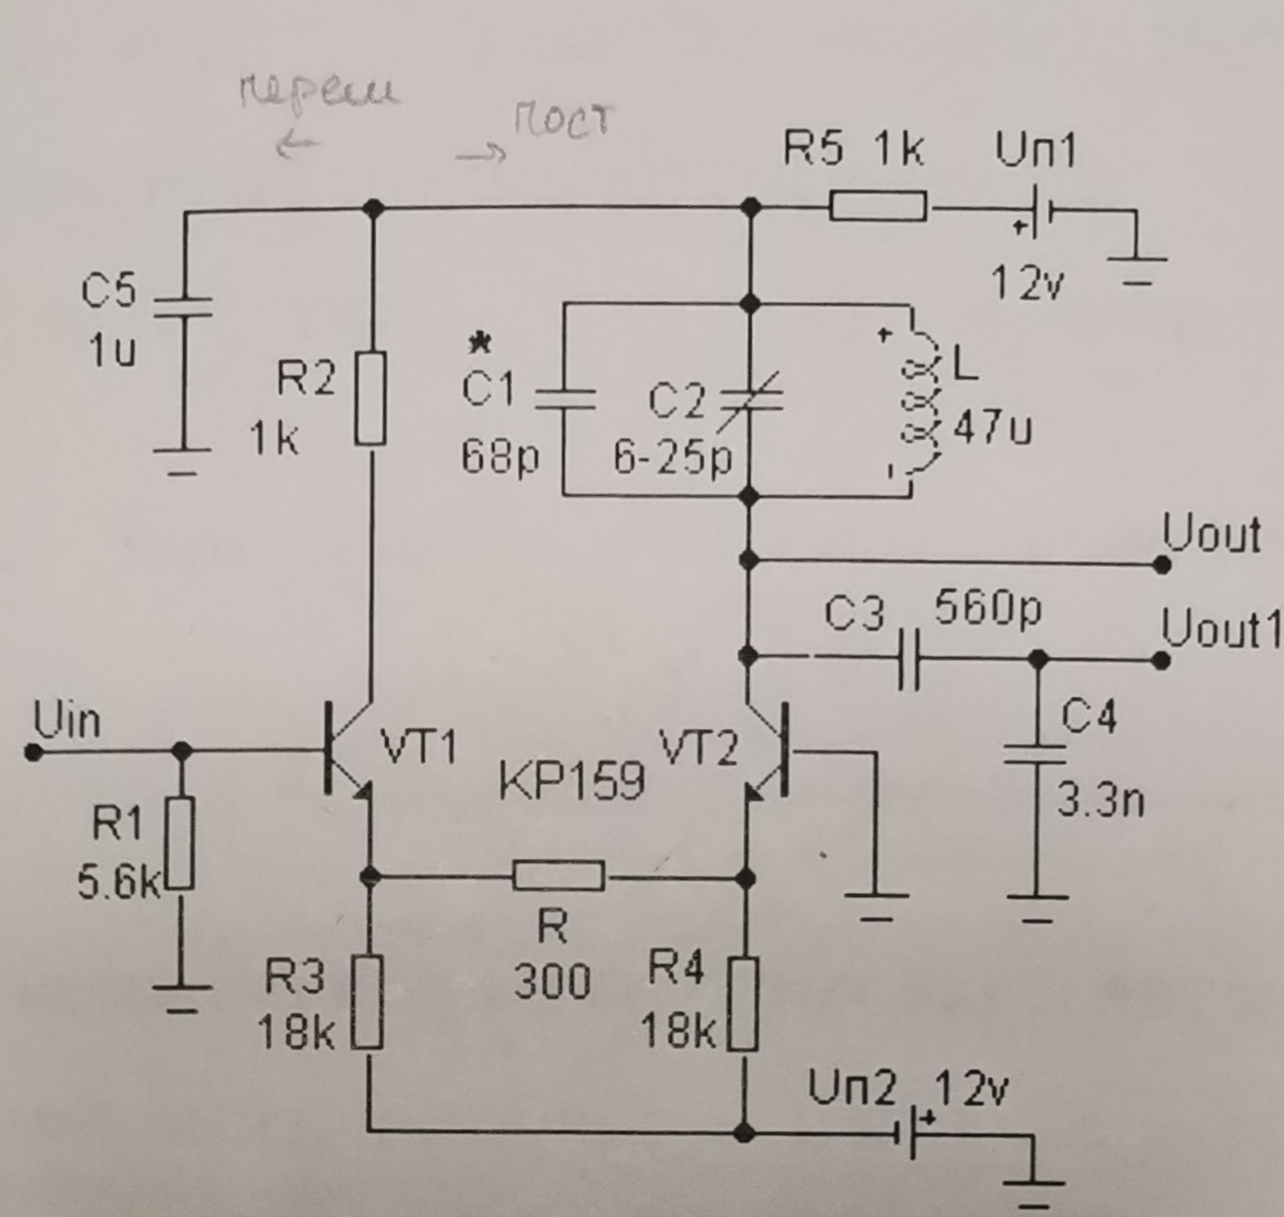
\includegraphics[width=0.8\linewidth]{pics/schm1.jpg}
    \caption{Cхема резонансного усилителя}
    \label{graph}
\end{figure}

\begin{enumerate}
    \item Напряжения $U_a$, $U_b$ связаны теоретическим сооотношением:
    \[ \beta_{теор}= \frac{U_a}{U_b} = \frac{C_3}{C_3 + C_4} \approx \frac{1}{7} \]

    \item При проведении эксперимента получили значения $U_a \approx 65,6 \text{ мВ}$, $U_b \approx 323 \text{ мВ}$.
    Таким образом, практическое значение несильно отличается:

    \[ \beta_{практ}= \frac{U_a}{U_b} = \frac{1}{4,90} \]

    \textbf{Причина расхождения теории и практики:} погрешность конденсаторов.

    \item С помощью конденсатора с переменной емкостью добиваемся частоты колебаний $f_k = 1 \text{ МГц}$. 

\end{enumerate}

\section{Кварцевый генератор с использованием последовательного резонанса кварца.}

\begin{figure}[h!]
    \centering
    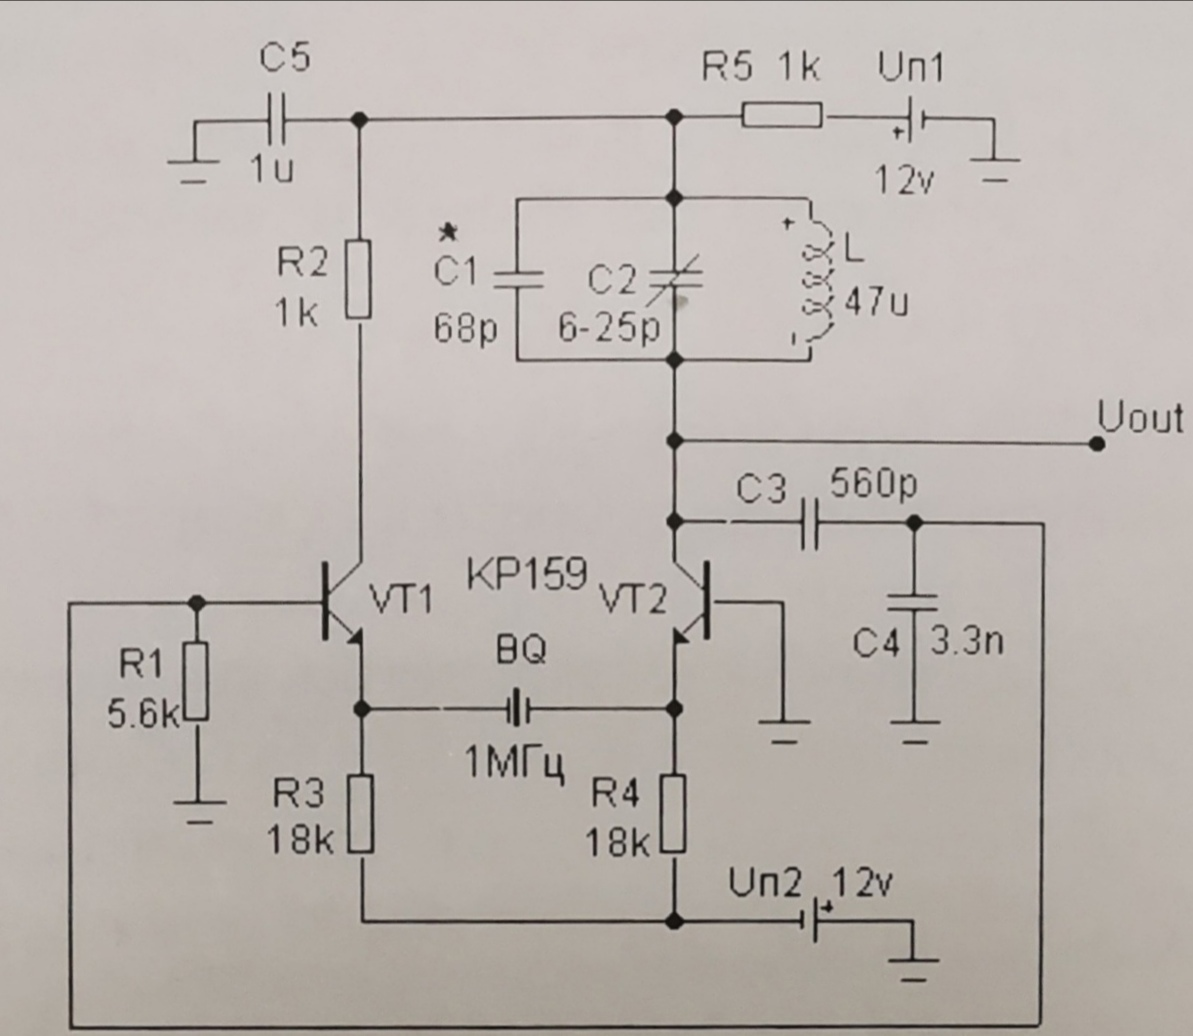
\includegraphics[width=0.8\linewidth]{pics/schm2.jpg}
    \caption{Cхема кварц. генератора с использованием последовательного резонанса кварца}
    \label{graph}
\end{figure}

\begin{enumerate}
    \item Замыкаем цепь обратной связью (т.е соединяем базу первого транзистора с проводом между $C_3$ и $C_4$).
    
    \item \textbf{Настройка контура:} установим вместо кварцевого резонатора переменный резистор. Ищем max $U_{out}$.
    
    $R_{пер} = 800 \text{ Ом} \: \Rightarrow \: 2r_e + R = 950 \text{ Ом}$ - сопротивление между эммитерами.  
    
    \item Рассчитаем добротность колебательного контура, используя формулу:
    \[ R_{экв} = Q\rho \]

    \[ \rho = \frac{1}{2\pi f C} = 300 \text{ Ом} \] 
    
    \[ K_{\beta} = \frac{1}{\beta} = \frac{R_{экв}}{2r_e + R} \]

    \[ {4,9} \approx 5 = \frac{R_{экв}}{950 \text{ Ом}} \Rightarrow R_{экв} \approx 4750 \text{ Ом} \]

    \[ Q = \frac{R_{экв}}{\rho} = \frac{4750 \text{ Ом}}{300 \text{ Ом}} \approx 15.8 \]

    \item Вместо резистора подключаем кварцевый генератор между эммитерами, последовательно ему - переменный резистор. Ищем max $U_{out}$, определяем $R_к$:
    \[ R_к = (800 - 355) \text{ Ом} = 445  \text{ Ом}\]

    \item Определим оставшиеся электрические параметры кварцевого резонатора:
    
    \textbf{Емкость}

    Последовательно кварцу подсоединяем $C_s = 120 \text{ Пф} \Rightarrow \Delta f_к = 25 \text{ Гц}$.
    Из формулы:

    \[ \frac{\Delta f_к}{f} = \frac{C_k}{2C_s} \: \Rightarrow \: C_{к} = \frac{\Delta f_к}{f} \cdot 2C_s = 6 \cdot 10^{-3} \text{ Пф} \]

    \textbf{Характеристическое сопротивление}

    Из формулы:

    \[ \rho_k = \sqrt{\frac{L_k}{C_k}} = \frac{1}{2\pi f_k C_k} = 26  \text{ МОм}\]

    \textbf{Добротность}
    
    Из формулы:

    \[ R_k = \frac{\rho_k}{Q_k} \: \Rightarrow \: Q = \frac{26 \cdot 10^6 \text{ Ом}}{455 \text{ Ом}} \approx 5.84 \cdot 10^{4} \]

    Согласно теории добротность кварцевого резонатора $\thicksim 10^{5}$.

    \item С кварцевым резонатором пронаблюдали стабильность частоты, изменяя питающее напряжение $U_{п2}$.
    
\end{enumerate}

\end{document}